\capitulo{6}{Trabajos relacionados}

La rehabilitación de pacientes con problemas físicos o mentales ha evolucionado en los últimos años, gracias a los avances tecnológicos, a un sistema de rehabilitación \textit{online}, que como se explico en la introducción del trabajo, permite habilitar estos sistemas de rehabilitación a pacientes que por diversas razones no pueden desplazarse a las consultas médicas a realizar esta rehabilitación para mejorar sus situación.

La aparición de las rehabilitaciones \textit{online} están permitiendo la automatización de estos sistemas. Gracias a herramientas de visión por computador permiten, sin la presencia de un médico especializado, dar una retroalimentación al paciente de los ejercicios que realiza.

A continuación, se van a comentar algunos de los proyectos, que como el proyecto que se ha desarrollado en este Trabajo Fin de Máster, han desarrollado un sistema que utiliza la visión por computador para mejorar las rehabilitaciones de pacientes.

\subsection{A Kinect-based system for cognitive rehabilitation exercises monitoring~\cite{kinectbasedsystem}}
En este \textit{paper} de la Universidad de Valladolid se puede observar el uso de técnicas de visión por computador para calcular características como el tiempo de reacción de los pacientes con algún problema físico o personas que confunden el lado derecho e izquierdo de su cuerpo, y seguir los movimientos del paciente.

Los ejercicios en los que se centra este proyecto se centran en movimientos de la mano hacia la cabeza, para ello utilizan la estimación de posición, en 3D, que les ofrece la cámara \textit{Kinect}. Kinect es una cámara desarrollada por \textit{Microsoft} que originalmente se diseñó desde un enfoque lúdico para la vídeo consola \textit{Xbox 360}, pero que ha terminado siendo una de las mejores cámaras para su uso en visión por computador~\cite{wiki:kinect}. Actualmente, con la nueva generación de la vídeo consola de \textit{Microsoft} (\textit{Xbox One}) salió en 2013 una nueva versión de su cámara \textit{Kinect}.

Para poder monitorizar estos ejercicios, se realiza una estimación y seguimiento de los rasgos faciales (ojos, nariz y orejas) y de las manos derecha e izquierda. Para realizar este proceso se utiliza la estimación de la posición dada por \textit{Kinect} y el uso de modelos predictivos como \textit{AdaBoost}~\cite{ada} para la detección de la cara, de la cual posteriormente se los rasgos faciales (el esqueleto proporcionado por \textit{Kinect} solo aporta la posición de la cabeza, no de los rasgos faciales).

En este proyecto se trabajó con vídeos de 640 × 480 píxeles con 13 fotogramas por segundo, con un tiempo medio de estimación de las posiciones necesarias de 79 milisegundos, realizado en Visual C++ en un dispositivo con un procesador de 3 GHz. La evaluación de los ejercicios se realiza de manera \textit{offline} una vez termina el ejercicio. 

Cabe destacar que este proyecto se desarrolló con la finalidad de ser incluido en \textit{GRADIOR}\footnote{\textit{GRADIOR}: \url{https://ides.es/gradior}}, plataforma virtual para la estimulación cognitiva, evaluación y rehabilitación neuropsicológica~\cite{gradior}.

\subsection{Computer Vision-Based Classification of Hand Grip Variations in Neurorehabilitation~\cite{hand}}
En este proyecto se realizó un sistema de visión por computador, que puede usarse con realidad virtual, para la clasificación de posturas de las manos en la rehabilitación de pacientes.

Para poder obtener mayor información para detectar correctamente la postura de la mano se utilizan dos cámaras, una que graba el lateral de la mano, y otra que graba la parte superior de ésta (figura~\ref{fig:hand}). Las cámaras capturan con una frecuencia de 15 fotogramas por segundo a una resolución de 352 $\times$ 288 píxeles.

\begin{figure}[h]
	\centering
	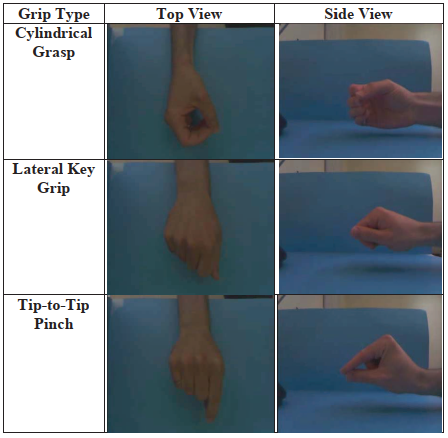
\includegraphics[width=0.5\textwidth]{hand}
	\caption{Ejemplos cámaras en rehabilitación de manos~\cite{hand}.}
	\label{fig:hand}
\end{figure}

Para el procesado de las imágenes se usa una librería de C++ llamada OpenCV. Con esta librería se quita el fondo de la imagen para dejar solo a la mano (con técnicas de comparación de colores, erosión y dilatación de la imagen). Sobre esta imagen procesada se obtiene:
\begin{itemize}
	\item Los siete \textit{Hu invariant moments} sobre una versión de escala de grises de la imagen~\cite{humingkuei2011}.
	\item Contorno de la mano.
	\item Contorno interior en los casos necesarios, cuando la mano hace la forma de un agujero.
\end{itemize}

La clasificación final de las posturas se realiza con estos datos utilizando \textit{k-Nearest Neighbors} (\textit{kNN}), calculado con los 20 vecinos más cercanos ($k=20$).

\subsection{A Computer Vision System for Virtual Rehabilitation~\cite{bonen}}
En este proyecto se utiliza la segunda versión de la cámara de \textit{Microsoft}, \textit{Kinect}, para la mejora en la estimación de la postura y el seguimiento del movimiento en personas con deficiencias motoras. Esta mejora se consigue utilizando las distintas cámaras de \textit{Kinect V2} y juntando toda esa información para obtener el mejor esqueleto posible en 3D. Además, el proyecto ha sido desarrollado para ser usado con realidad virtual con \textit{Oculus RIFT 2 HMD}.

Este proyecto destaca por el uso de 4 \textit{Kinect V2} puestas en las esquinas de la habitación conectadas a un \textit{Intel Next Unit of Computing} (\textit{NUC}) que permite preprocesar las imágenes, solo unos pocos puntos son mandados al ordenador maestro (\textit{Master PC}) para crear el esqueleto (figura~\ref{fig:4kinects}).

\begin{figure}[h]
	\centering
	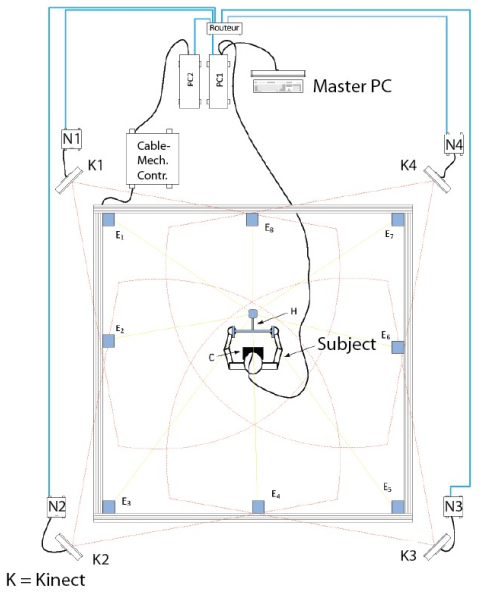
\includegraphics[width=0.5\textwidth]{4kinect}
	\caption{Disposición \textit{Kinects V2}(\textit{K}), \textit{NUC}(\textit{N}) y el \textit{Master PC}~\cite{bonen}.}
	\label{fig:4kinects}
\end{figure}

En el \textit{paper} los creadores comentan que la estimación de la posición de \textit{Microsoft} es muy buena, pero que al tener 4 \textit{Kinects V2} se tiene que juntar y aplicar unos filtros para el correcto funcionamiento.

Además, en el \textit{paper} se describen dos formas de ejecutar la estimación de la posición desarrollada, una versión en <<tiempo real>> que permite mandar la información del esqueleto directamente a las \textit{Oculus}, y una versión \textit{offline} de mayor precisión pero con la necesidad de un postprocesado de la información obtenida.


\subsection{Conclusiones}
Todos estos proyectos, cada uno orientado y elaborado de una forma distinta, muestran lo valioso que puede llegar a ser la introducción de la tecnología en la rehabilitación de pacientes con problemas físicos e incluso mentales. Este valor añadido ofrece, además de una reducción en costes y en intervención humana, una mejoría en la vida de los pacientes ya que realizan más rehabilitaciones que hacen sus vidas más llevaderas~\cite{motiv}.
